\subsection{Boss and stealing employee}

\paragraph{Answers}
\subsubsection{Analyse this game using backward induction.}
\begin{figure}[ht]
    \centering
    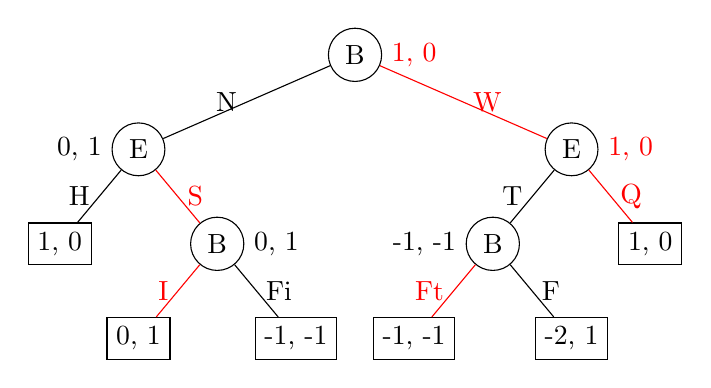
\begin{tikzpicture}[
        grow                    = down,
        % sibling distance        = 10em,
        level 1/.style          = {sibling distance=5.5cm},
        level 2/.style          = {sibling distance=2cm},
        level 3/.style          = {sibling distance=2cm},
        level distance          = 1.2cm,
        edge from parent/.style = {draw, edge from parent path={(\tikzparentnode) -- (\tikzchildnode)}},
        %sloped
      ]
        \node[circle, black,draw, label={[red]right: 1, 0}] {B}
            child {
                node[circle, draw, label={[black]left: 0, 1}] {E}
                child{
                        node[draw] {1, 0} 
                        edge from parent [left, black] node {H}
                    }
                child {
                    node[circle, draw, label={[black]right: 0, 1}] {B}
                    child{
                        node[draw, black] {0, 1}
                        edge from parent [left, red] node {I}
                    }
                    child{
                        node[draw, black] {-1, -1}
                        edge from parent [right, black] node {Fi}
                    }
                    edge from parent [right, red] node {S}
                }
                edge from parent [left, black] node {N}
            }
            child {
                node[circle, black, draw, label={[red]right: 1, 0}] {E}
                child {
                    node[circle, black, draw, label={[black]left: -1, -1}] {B}
                    child {
                        node [draw] {-1, -1}
                        edge from parent [left, red] node {Ft}
                    }
                    child {
                        node [draw] {-2, 1}
                        edge from parent [right, black] node {F}
                    }
                    edge from parent [left, black] node {T}
                }
                child {
                    node [draw, black] {1, 0}
                    edge from parent [right, red] node {Q}
                }
                edge from parent [right, red] node {W}
            };
    \end{tikzpicture}
\end{figure}
The backwards induction shows, that the rational move for the Boss would be to give a Warning
and then for the employee to quit steeling.



\subsubsection{What are the pure actions for the two players (boss and employee)? Construct the normal
form matrix.}


\begin{table}[H]
  \centering
  \begin{tabular}{|l|l|l|l|l|l|l|l|}
    \hline
    & HT                                    & HQ                            & ST   & SQ   \\ \hline
    NIFt  & \underline{1}, 0                & \underline{1}, 0              & \underline{0}, \underline{1}   & 0, \underline{1}             \\ \hline
    NIF   & \underline{1}, 0                & \underline{1}, 0              & \underline{0}, \underline{1}   & 0, \underline{1}             \\ \hline
    NFiFt & \underline{1}, \underline{0}    & \underline{1}, \underline{0}  & -1, -1                         & -1, -1                       \\ \hline
    NFiF  & \underline{1}, \underline{0}    & \underline{1}, \underline{0}  & -1, -1                         & -1, -1                       \\ \hline
    WIFt  & -1, -1                          & \underline{1}, \underline{0}  & -1, -1                         & \underline{1}, \underline{0} \\ \hline
    WIF   & -2, \underline{1}               & \underline{1}, 0              & -2, \underline{1}              & \underline{1}, 0             \\ \hline
    WFiFt & -1, -1                          & \underline{1}, \underline{0}  & -1, -1                         & \underline{1}, \underline{0} \\ \hline
    WFiF  & -2, \underline{1}               & \underline{1}, 0              & -2, \underline{1}              & \underline{1}, 0             \\ \hline


  \end{tabular}
  \caption{Normal Form for the Boss and stealing employee game.}
  \label{lt2}
\end{table}


\subsubsection{Use this matrix to identify all the pure Nash equilibria of the normal form game.}

\begin{table}[H]
  \centering
  \begin{tabular}{|l|l|l|l|l|l|l|l|}
      \hline
      & HT                           & HQ                           & ST                           & SQ                           \\ \hline
      NIFt  & \underline{1}, 0             & \underline{1}, 0             & \fbox{\underline{0}, \underline{1}} & 0, \underline{1}             \\ \hline
      NIF   & \underline{1}, 0             & \underline{1}, 0             & \fbox{\underline{0}, \underline{1}} & 0, \underline{1}             \\ \hline
      NFiFt & \fbox{\underline{1}, \underline{0}} & \fbox{\underline{1}, \underline{0}} & -1, -1 & -1,-1 \\ \hline
      NFiF  & \fbox{\underline{1}, \underline{0}} & \fbox{\underline{1}, \underline{0}} & -1, -1 & -1, -1                       \\ \hline
      WIFt  & -1, -1                       & \fbox{\underline{1}, \underline{0}} & -1, -1                       & \fbox{\underline{1}, \underline{0}} \\ \hline
      WIF   & -2, \underline{1}            & \underline{1}, 0             & -2, \underline{1}            & \underline{1}, 0             \\ \hline
      WFiFt & -1, -1                       & \fbox{\underline{1}, \underline{0}} & -1, -1                       & \fbox{\underline{1}, \underline{0}} \\ \hline
      WFiF  & -2, \underline{1}            & \underline{1}, 0             & -2, \underline{1}            & \underline{1}, 0             \\ \hline


  \end{tabular}
  \caption{Pure Nash Equilibria of the normal form game.}
  \label{lt3}
\end{table}

\subsubsection{Determine the subgame-perfect equilibrium (equilibria?) by eliminating all the Nash equilibria that fail
to induce a NE in subgame}
\begin{figure}[ht]
    \centering
    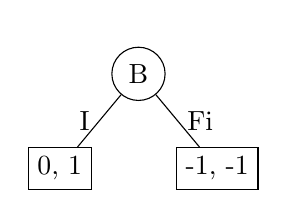
\begin{tikzpicture}[
        grow                    = down,
        % sibling distance        = 10em,
        level 1/.style          = {sibling distance=2cm},
        level distance          = 1.2cm,
        edge from parent/.style = {draw, edge from parent path={(\tikzparentnode) -- (\tikzchildnode)}},
        %sloped
      ]
        \node[circle, black,draw, label={}] {B}
                    child{
                        node[draw, black] {0, 1}
                        edge from parent [left, black] node {I}
                    }
                    child{
                        node[draw, black] {-1, -1}
                        edge from parent [right, black] node {Fi}
                    };
    \end{tikzpicture}
    \caption{Subgame 1 with NE (I).}
\end{figure}

\begin{figure}[ht]
    \centering
    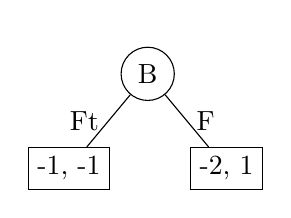
\begin{tikzpicture}[
        grow                    = down,
        % sibling distance        = 10em,
        level 1/.style          = {sibling distance=2cm},
        level distance          = 1.2cm,
        edge from parent/.style = {draw, edge from parent path={(\tikzparentnode) -- (\tikzchildnode)}},
        %sloped
      ]
        \node[circle, black,draw, label={}] {B}
                    child{
                        node[draw, black] {-1, -1}
                        edge from parent [left, black] node {Ft}
                    }
                    child{
                        node[draw, black] {-2, 1}
                        edge from parent [right, black] node {F}
                    };
    \end{tikzpicture}
    \caption{Subgame 2 with NE (Ft).}
\end{figure} 

\begin{figure}[ht]
    \centering
    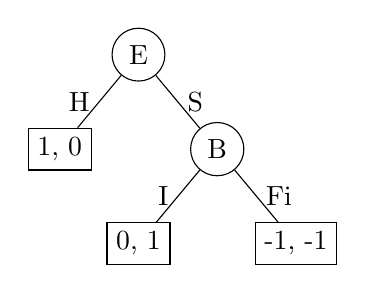
\begin{tikzpicture}[
        grow                    = down,
        % sibling distance        = 10em,
        level 1/.style          = {sibling distance=2cm},
        level 2/.style          = {sibling distance=2cm},
        level distance          = 1.2cm,
        edge from parent/.style = {draw, edge from parent path={(\tikzparentnode) -- (\tikzchildnode)}},
        %sloped
      ]
        \node[circle, draw, label={[black]left:}] {E}
                child{
                        node[draw] {1, 0} 
                        edge from parent [left, black] node {H}
                    }
                child {
                    node[circle, draw, label={[black]right:}] {B}
                    child{
                        node[draw, black] {0, 1}
                        edge from parent [left, black] node {I}
                    }
                    child{
                        node[draw, black] {-1, -1}
                        edge from parent [right, black] node {Fi}
                    }
                    edge from parent [right, black] node {S}
                };
    \end{tikzpicture}
    \caption{Subgame 3 with NE (FtQ).}
\end{figure}

\begin{figure}[ht]
    \centering
    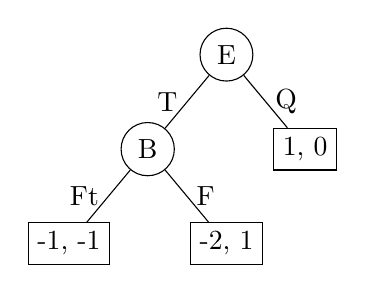
\begin{tikzpicture}[
        grow                    = down,
        % sibling distance        = 10em,
        level 1/.style          = {sibling distance=2cm},
        level 2/.style          = {sibling distance=2cm},
        level distance          = 1.2cm,
        edge from parent/.style = {draw, edge from parent path={(\tikzparentnode) -- (\tikzchildnode)}},
        %sloped
      ]
        \node[circle, black, draw, label={[red]right:}] {E}
                child {
                    node[circle, black, draw, label={[black]left:}] {B}
                    child {
                        node [draw] {-1, -1}
                        edge from parent [left, black] node {Ft}
                    }
                    child {
                        node [draw] {-2, 1}
                        edge from parent [right, black] node {F}
                    }
                    edge from parent [left, black] node {T}
                }
                child {
                    node [draw, black] {1, 0}
                    edge from parent [right, black] node {Q}
                };
    \end{tikzpicture}
    \caption{Subgame 4 with NEs (IS, FiH).}
\end{figure}

Figures 2-5 show the subgames and mention their NEs. The only subgame-perfect equilibrium is (WIFtSQ), as it is the only one that induces a NE in each subgame.

\subsubsection{Compare to the solution based on backward induction.}
The solutions are identical. The subgame-perfect equilibrium (WIFtSQ) will result in the Boss picking (W) and the employee then (Q), which is the choice path determined by backward induction.